
% =====================
% Chapter 2: Basics (Revised with section explanations)
% Audience: Architecture students new to coding
% =====================

\h{Basics of Python: Comments, Literals, Variables, and Layout}
Before an architect/engineer can design a complex building, they must first understand the fundamental language of architectural/structural drawings: lines, symbols, and annotations. A script, like a blueprint, also has its own fundamental language. In Python, this language is built from a few core components that work together to create clear, readable, and functional instructions. This chapter will introduce you to these foundational elements: comments, which are notes for humans; literals, the raw data your program works with; variables, the containers that store that data; and layout, the rules of spacing and indentation that give your code structure and meaning. Mastering these basics is the first and most critical step in learning to write effective code.
\medskip

\begin{NoteBox}
\textbf{About this chapter.} Everyday building blocks for ARC500: how to write useful comments, what a \emph{literal} is, core text/number types, and how Python treats lines and indentation. Examples use short, unit-aware code for built-environment tasks.
\end{NoteBox}
\medskip

\begin{tcolorbox}[% passing options here
    title=Focus of this chapter:,
    colframe=orange,
    colback = white,
%    colback=orange!40!yellow!30, % think of mixing 2 colors with sliders
    arc=2mm % sharp corners
 ]

\begin{itemize}
    \item Comments: Use \c{#} to record assumptions, decisions, and intent in code; distinguish between short comments and docstrings for modules/functions.
    \item Literal constants: Learn how numbers (\c{5}, \c{1.23}), text (\c{'Lobby'}, \c{"GLT beam"}), and special values (\c{True}, \c{False}, \c{None}) appear directly in code.
    \item Numbers (\c{int}, \c{float}): Work with whole numbers and decimal values; understand floating-point quirks and how to format results with \c{round()}.
    \item Arithmetic operators: Apply the operators you will use most: addition (\c{+}), subtraction (\c{-}), multiplication (\c{*}), division (\c{/}, \c{//}), remainder (\c{%}), and exponentiation (\c{**}).
    \item Strings (\c{str}): Create text with single, double, or triple quotes; slice and index strings; and format with \c{.format()} or f-strings for clear reports.
    \item Variables and assignment: Bind names to values with \c{=}, rebind them as needed, and use multiple assignment for concise code.
    \item String variables and concatenation: Combine text values, repeat with \c{*}, and convert numbers with \c{str()} or \c{int()} when mixing text and numbers.
    \item Deleting variables: Remove bindings or list items with \c{del}, and understand how names, not objects, are deleted.
    \item Identifiers and naming style: Follow ARC500 conventions: lowercase\_with\_underscores, include units (\c{span_m}, \c{load_kpa}), and avoid shadowing built-ins like \c{list}.
    \item Everything is an object: Use \c{type(x)} to inspect runtime types and preview the idea of truthiness in conditions.
    \item Lines and indentation: Distinguish logical vs. physical lines, avoid semicolons, prefer implicit line joining inside \c{()} or \c{[]}, and use 4-space indentation.
    \item Worked examples and labs: Apply these basics to small tasks: area checks, cost estimates, and string-formatted reports.
    \item Common mistakes and pitfalls: Spot and fix issues like mixing strings and numbers, shadowing built-ins, or misusing \c{is} vs. \c{==}.
\end{itemize}
\end{tcolorbox}

\hh{How Python Executes Your Code (Top -> Bottom)}

\begin{NoteBox}
Python runs your file \emph{from the first line to the last, one line at a time}.
For Chapter 2, think “straight line.” Other cases (like \c{if} decisions or loops) will come later.
\end{NoteBox}

\hh{Sequential execution (the normal case)}
\code{c02_seq}{python}{
    print("1) Start")
    print("2) Load site data")
    print("3) Compute areas")
    print("4) Done")
}{Runs line by line}

\textit{Order of output:} 1, then 2, then 3, then 4.

\hh{Comments and blank lines are ignored}
\code{c02_comments}{python}{
    print("Start")
    # This is a comment for the human reader.
    # It does not affect execution.
    print("Next step")   # Inline comments are fine, too.

    print("Blank lines don't change the order.")
    print("End")
}{Comments/blank lines don't execute}

\hh{Preview: Indentation (why spacing matters)}
A block begins after a line that ends with \c{:} and continues while the indentation level stays the same.
(We will fully cover \c{if} and loops later—this is just to show indentation.)

\code{c02_indent_preview}{python}{
    rooms = 3
    if rooms > 0:
        print("We have rooms to process.")   # inside the indented block
    print("Continuing...")                    # back at top level
}{Indentation creates a block}
\textit{That’s all you need now: top -> bottom. Other execution patterns will be discussed later.}

\hh{Comments: what they are and how to use them}

Why and how to write comments that capture assumptions, decisions, and intent. Comments start with \c{\#} and everything to the right is ignored by Python. Prefer short, precise notes over narrative paragraphs.


A comment is text the interpreter ignores. Use comments to capture assumptions, decisions, and intent---the "why," not just the "how." A line that begins with \# is a comment; anything after \# on a line is also ignored.

\code{c02_comment_single}{python}{
    # Project: Studio Annex quick checks
    print("ARC500 room check")   # one-line description of the script
    # Assumption: minimum room area is 9 m^2 per studio guideline
    min_area_m2 = 9
}{Single-line and end-of-line comments.}

\hhh{Temporarily disabling code while testing}

Turning a line off by commenting it out to focus on a small part of your script. Re-enable when done.


You can comment out a statement while you test:

\code{c02_comment_disable}{python}{
    # print("Draft: extra debug line")
    print("Ready")
}{Commenting out a line to prevent execution.}

\hhh{Multi-line comments? Use one hash per line}

Python has no dedicated multi-line comment syntax. Use one \c{#} per line for multi-line notes. Triple-quoted strings are for documentation, not general comments.


Python has no special multi-line comment syntax. Write a \c{#} on each line for multi-line notes.

\code{c02_comment_multiline}{python}{
    # This script reads room data,
    # flags undersized rooms, and
    # prints a short report.
    pass
}{Multi-line notes with \# each line.}

\begin{NoteBox}
\textbf{Docstrings vs. comments.} An unassigned triple-quoted string \c{\"\"\"like this\"\"\"} is a string literal the interpreter creates and immediately discards. It behaves like a block comment, but reserve triple-quoted strings for docstrings (placed at the start of a module or after \c{def}).
\end{NoteBox}

\hh{Literal constants: values written directly in code}

\noindent How to recognize and use literals: numbers, strings, booleans, \c{None}, and collection literals. Literals evaluate to themselves; no name lookup.


A \textbf{literal} is a fixed value written directly in your source (e.g., \c{42}, \c{3.14}, \c{"Lobby"}). Literals evaluate to themselves and do not require looking up a name. You will use:

\items{
¤ \textbf{Numeric literals:} integers (\c{42}), floats (\c{3.14}), with optional digit separators (\c{8_804_190}). Bases: \c{0b1010}, \c{0o17}, \c{0xFF}.
¤ \textbf{String literals:} text in quotes---single, double, or triple for multi-line.
¤ \textbf{Boolean literals:} \c{True} and \c{False}.
¤ \textbf{Special singleton:} \c{None} to mean "no value yet."
¤ \textbf{Collection literals:} list \c{[]}, tuple \c{()}, dict \c{{}}, set \c{{1, 2}} (\c{set()} for empty set). Dictionary and set look similar in Python because both use curly braces \c{{}}, but they are actually very different data types. Details will be covered in Chapter 3.
}

\begin{figure}[htp!]
  \centering
  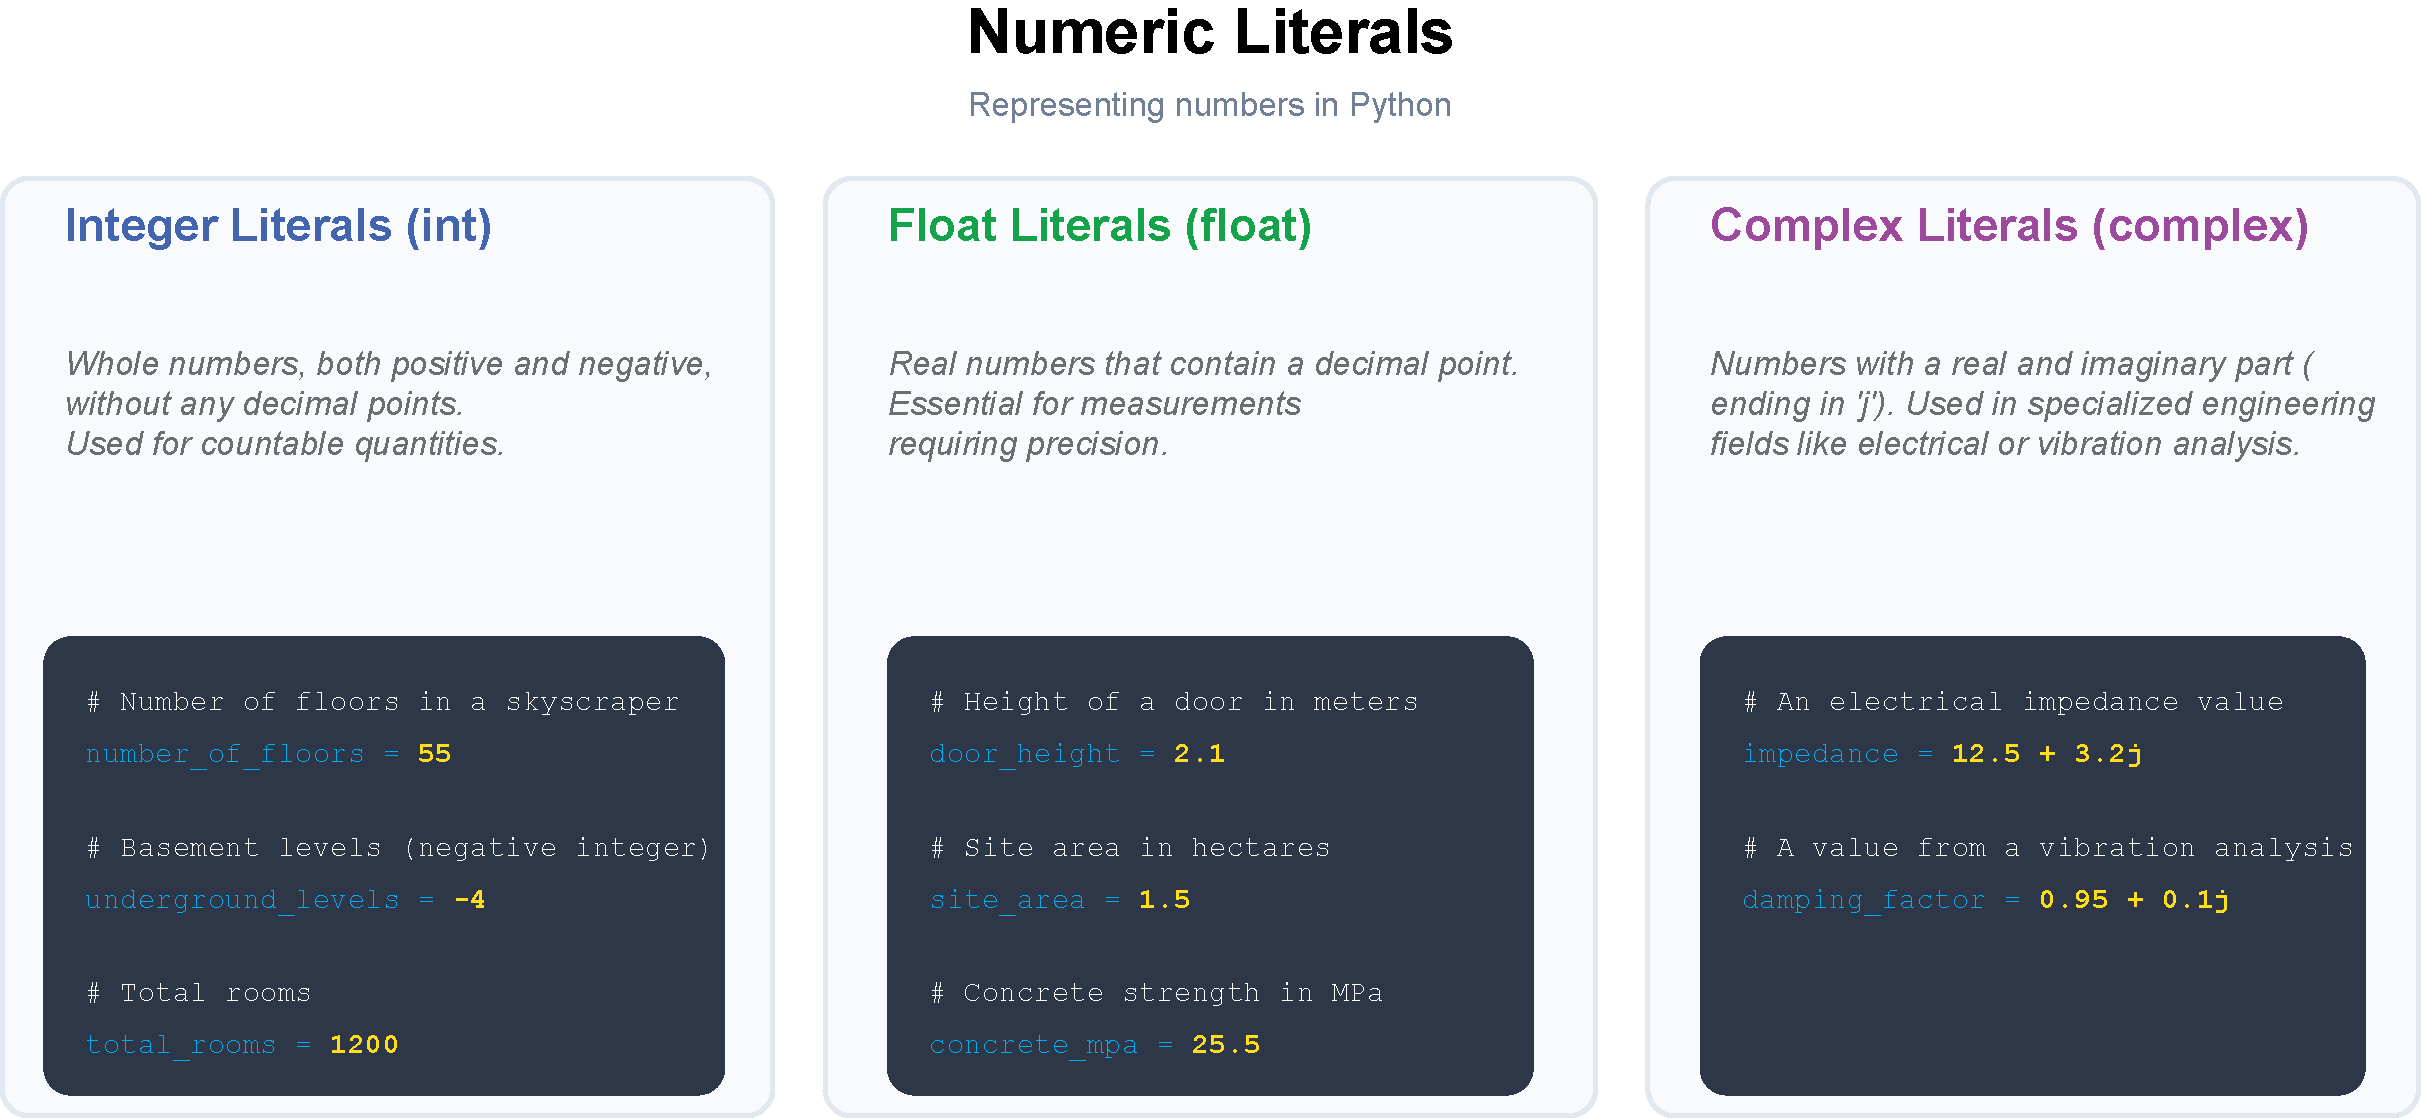
\includegraphics[width=0.9\linewidth,keepaspectratio]{Figures/Literals/Numeric_Literals.pdf}
  \caption{Numeric Literals.}
  \label{fig:Numeric Literals}
\end{figure}

\begin{figure}[htp!]
  \centering
  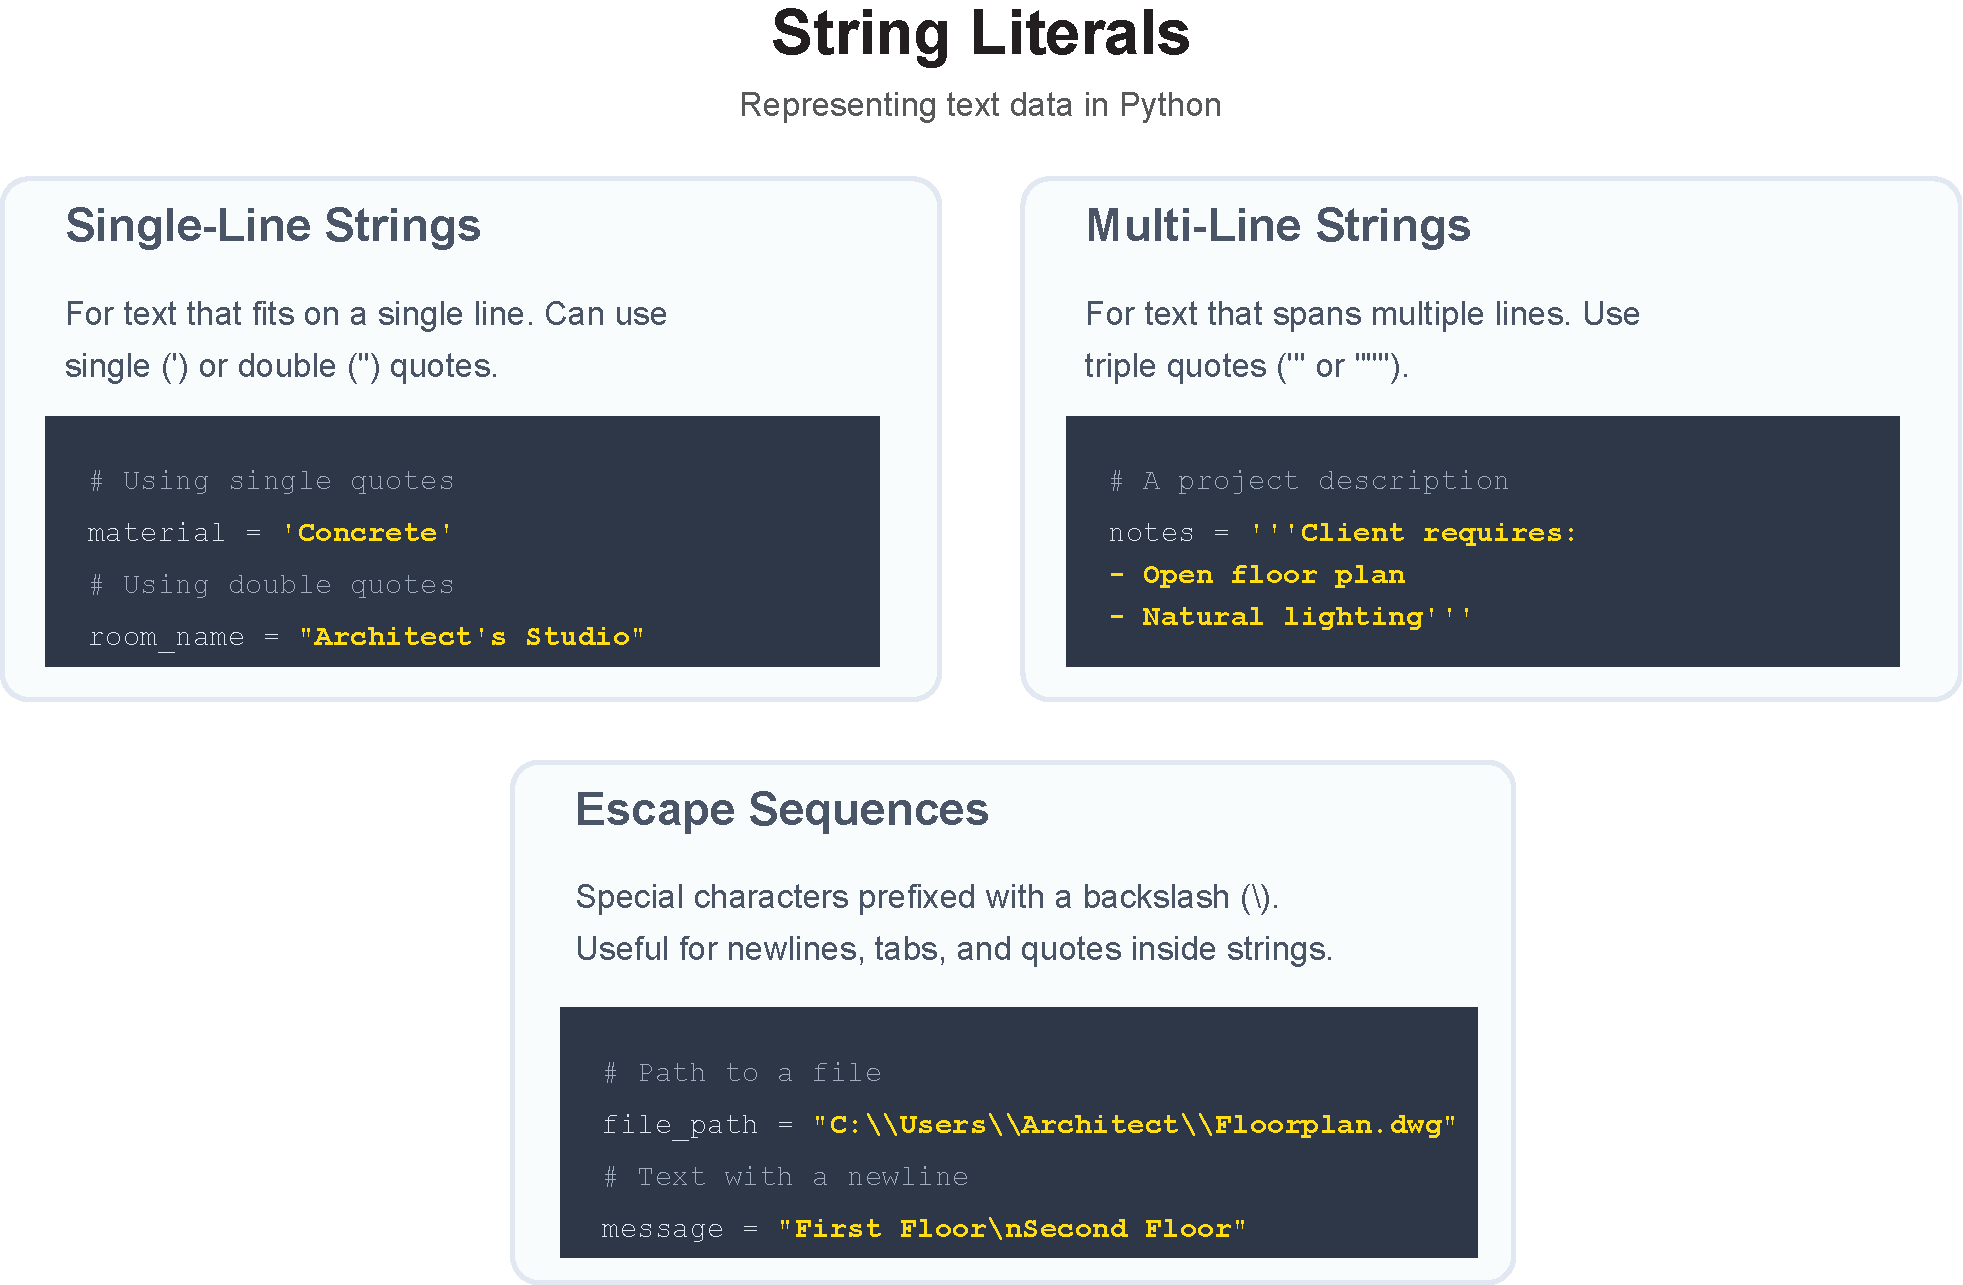
\includegraphics[width=0.80\linewidth,keepaspectratio]{Figures/Literals/String_Literals.pdf}
  \caption{String Literals.}
  \label{fig:String Literals}
\end{figure}

\begin{figure}[htp!]
  \centering
  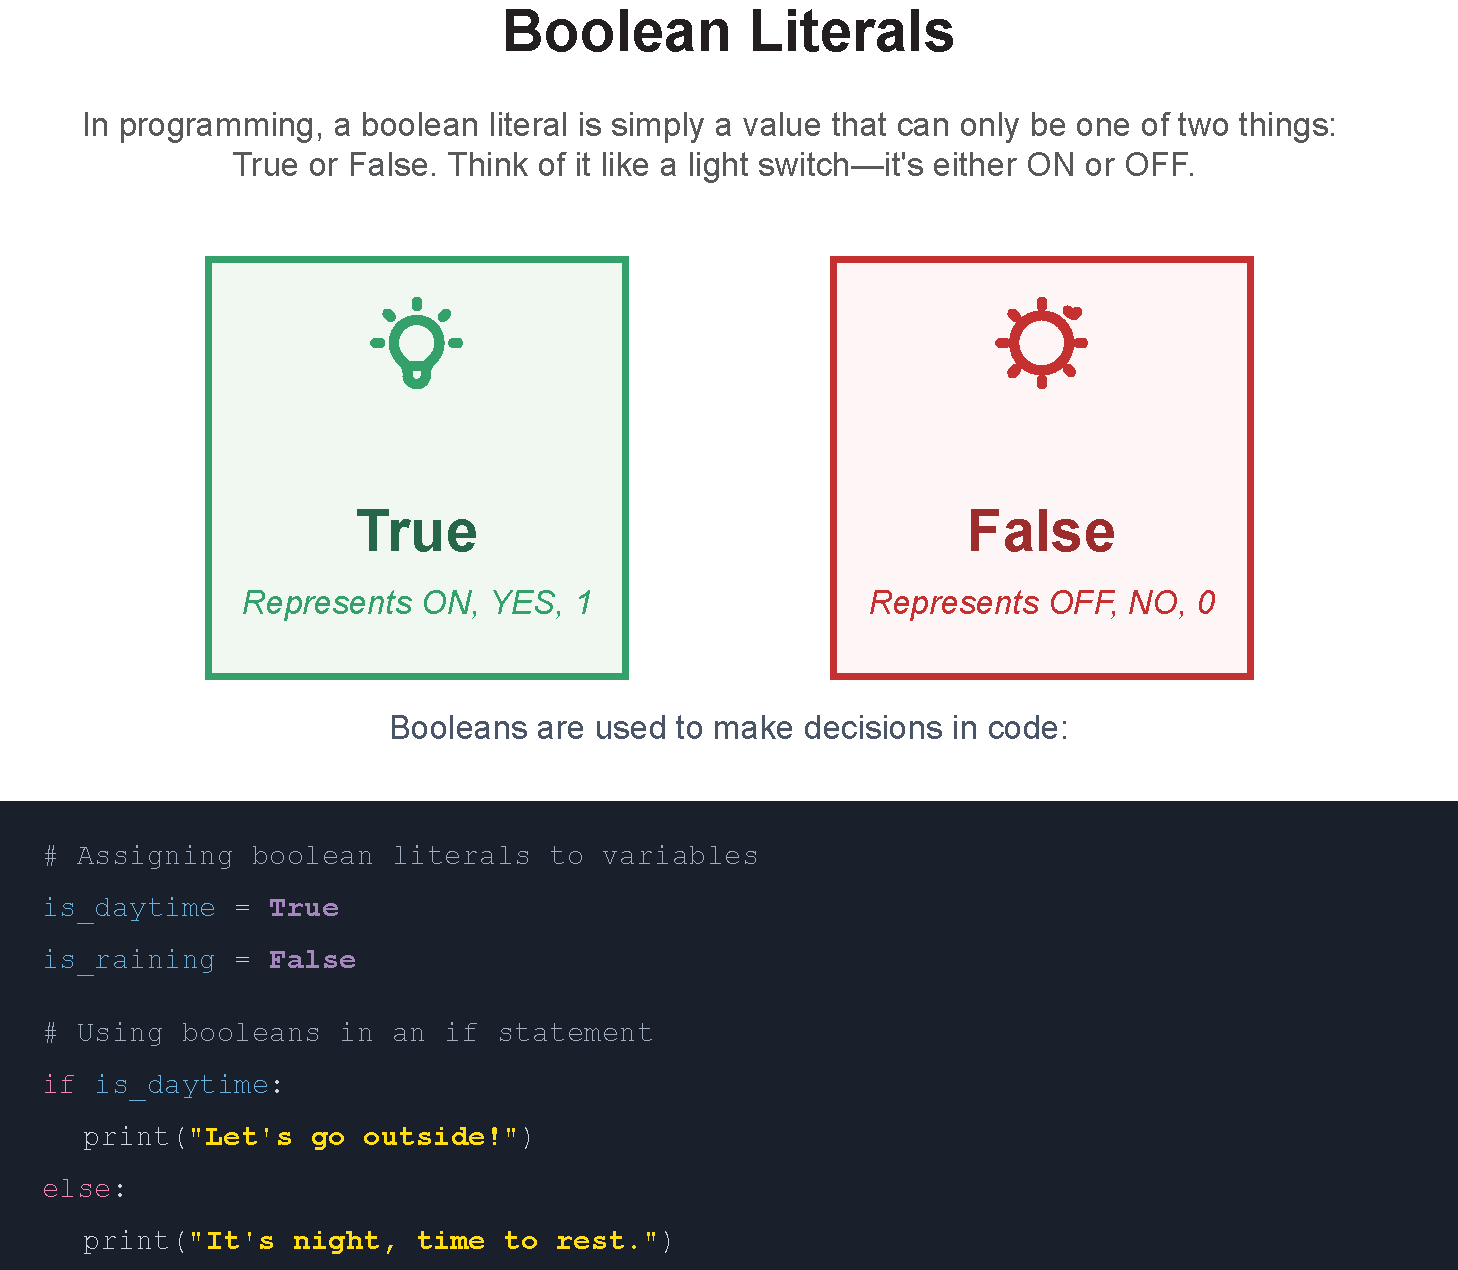
\includegraphics[width=0.80\linewidth,keepaspectratio]{Figures/Literals/Boolean_Literal.pdf}
  \caption{Boolean Literals.}
  \label{fig:Boolean Literals}
\end{figure}

\begin{figure}[htp!]
  \centering
  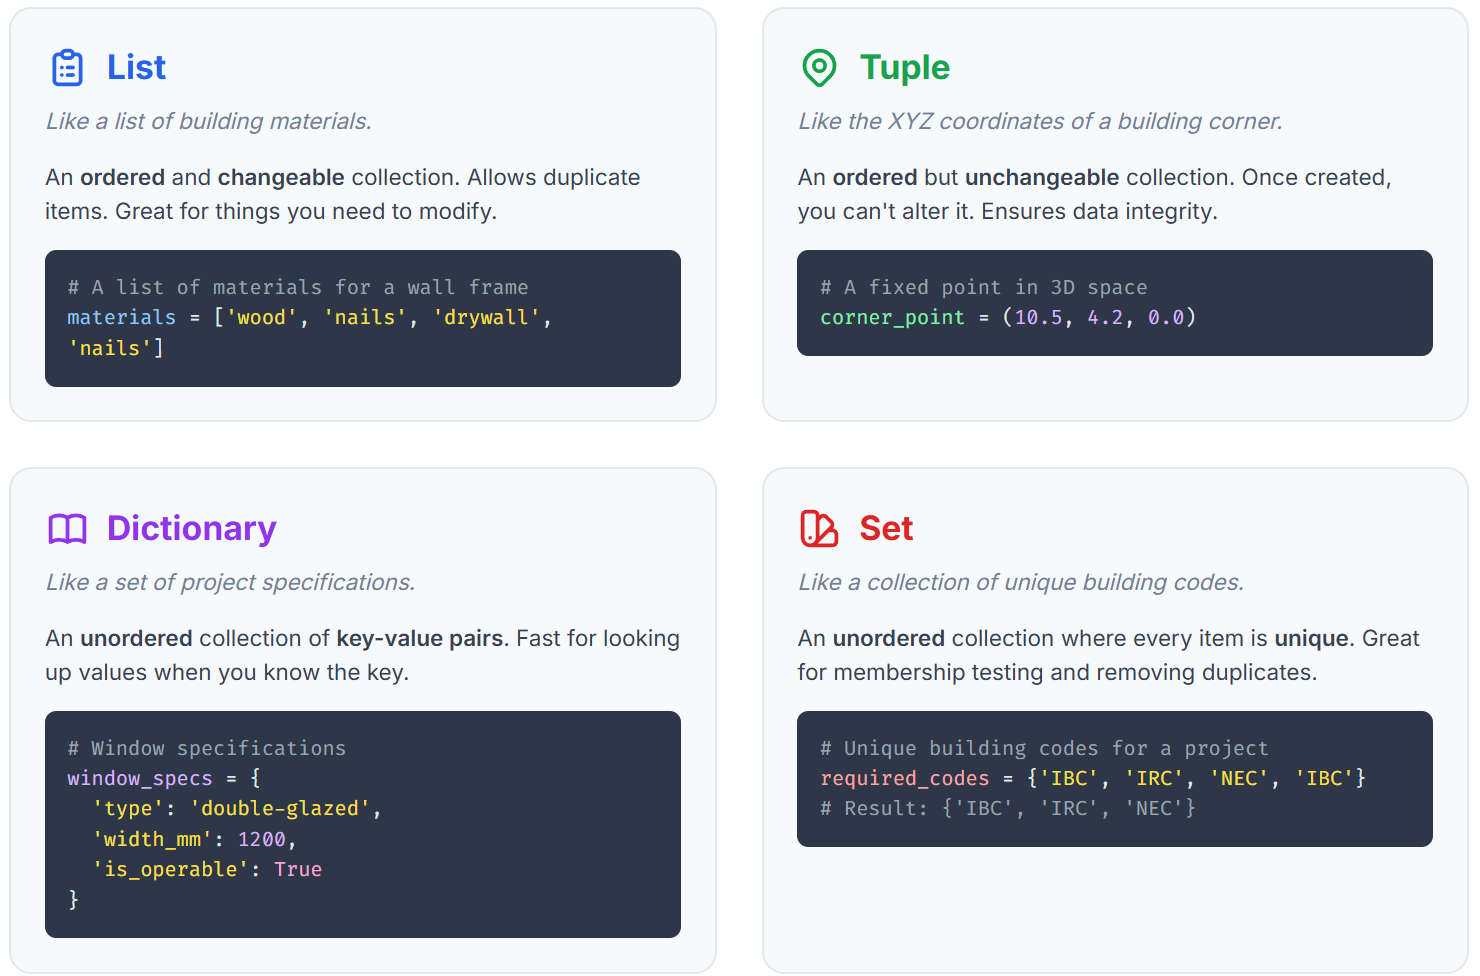
\includegraphics[width=0.85\linewidth,keepaspectratio]{Figures/Literals/Collection literals.png}
  \caption{Collection Literals.}
  \label{fig:Collection Literals}
\end{figure}

\code{c02_literals_overview}{python}{
    # Numbers
    levels = 6                # int
    bay_spacing_m = 7.2       # float
    pop = 8_804_190           # underscores improve readability
    mask = 0xFF               # hexadecimal 255

    # Strings
    title = "Lobby"
    note = \"\"\"Multi-line note:
    Unit: m^2; Code: 'R-2'.\"\"\"

    # Boolean, None
    open_to_public = True
    phase = None              # not set yet

    # Collections (literals)
    floors = [1, 2, 3]                      # list
    point = (15.5, 30.2, 0.0)               # tuple (immutable)
    mat_density = {"steel": 7850, "wood": 600}  # dict
    unique_levels = {0, 1, 2}               # set
}{Common literal forms.}

\begin{NoteBox}
\textbf{Literal vs constructor.} \c{[]} always creates a new list literal; \c{list()} calls the name \c{list}, which could in theory be rebound. Literals are part of the language syntax and reliably create the intended objects.
\end{NoteBox}

\hh{Numbers and formatting}


\noindent Basic arithmetic with floats and how to format results for reports using f-strings or \c{round()}.



\code{c02_numbers}{python}{
    span = 7.2
    udl_kn_per_m = 3.5
    total_line_load = span * udl_kn_per_m
    print(f"Span: {span} m | Line load: {total_line_load:.1f} kN/m")
}{Basic arithmetic and formatted printing.}

\hhh{Binary floating point caveat}


\noindent Why some decimals are not exact in binary (e.g., 0.1 + 0.2). For display, round or format; for money, prefer integers of cents or \c{decimal.Decimal}.


Some decimals are inexact in binary (e.g., \c{0.1 + 0.2}). Round for display when needed.

\code{c02_float_round}{python}{
    print(0.1 + 0.2)             # 0.30000000000000004
    print(round(0.1 + 0.2, 2))   # 0.30 for readability
}{Display rounding.}

\begin{NoteBox}
\textbf{Money caution.} For currency, prefer integer cents or the \c{decimal} module.
\end{NoteBox}

\hh{Strings: single, double, triple, and raw}

\noindent Common string forms, multi-line strings, and raw strings for paths. Strings are immutable; building a new string returns a new object.


Use single/double quotes for short text; triple quotes for multi-line. Raw strings (prefix \c{r}) disable backslash escapes---helpful for Windows paths.

\code{c02_strings}{python}{
    m1 = 'Lobby'
    m2 = "What's your name?"
    note = """This is multi-line.
    Unit: m^2; Code: 'R-2'."""
    raw = r"C:\studio\ARC500\data" # Raw string (r"...") keeps backslashes as they are. Useful for file paths in Windows without doubling every slash.
    # Print several variables in one line.
    # sep=" | " means each value is separated by a vertical bar with spaces around it.
    print(m1, m2, raw, sep=" | ") #Outcome: Lobby | What's your name? | C:\studio\ARC500\data
}{Common string forms.}

\hhh{String indexing}
Strings are sequences of characters. Think of a string as a row of rooms, each with a unique number. Python gives each character (room) two numbers: a positive index starting from the left (0) and a negative index starting from the right (-1)
\begin{figure}[htp!]
  \centering
  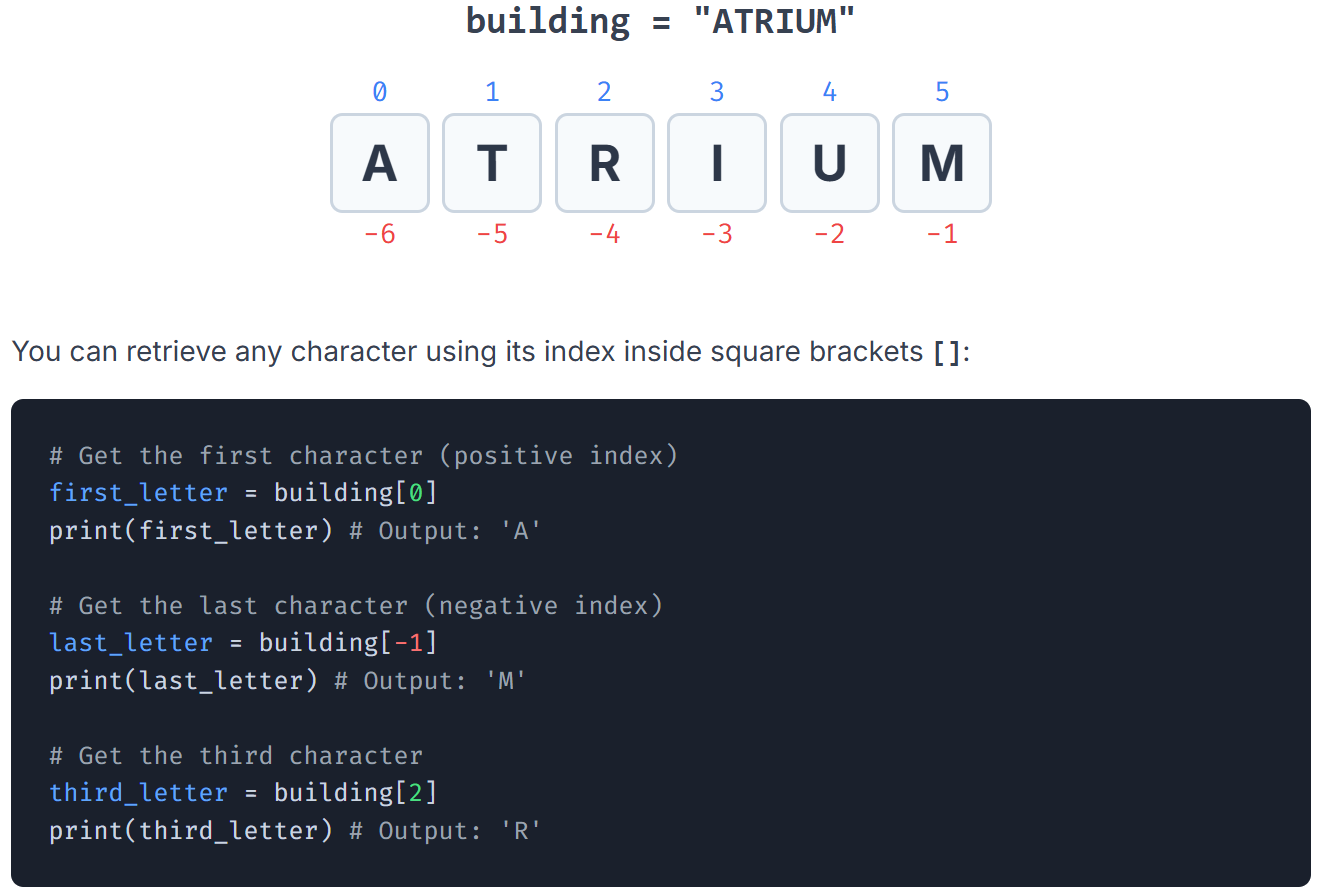
\includegraphics[width=0.85\linewidth,keepaspectratio]{Figures/Literals/String indexing.png}
  \caption{String indexing: accessing individual characters in a string.}
  \label{fig:Numeric Literals}
\end{figure}


\hhh{String Multiplication}

\noindent 
In Python, you can multiply a string by an integer to repeat it.  
This is useful for formatting, simple patterns, or quick placeholders.

\code{c02_strmult}{python}{
    print("ARC" * 3)          # Repeat a word
    # Output: ARCARCARC

    print("-" * 10)           # Create a line separator
    # Output: ----------

    print("Room " * 4)        # Repeat with space at the end
    # Output: Room Room Room Room 

    # Using variables
    label = "Beam "
    count = 5
    print(label * count)    # Output: Beam Beam Beam Beam Beam 
}{Repeating strings with multiplication.}


\hhh{Escape Sequences}

Escape sequences let you include special characters inside strings.  
\items{
¤ \c{\n} --- newline (line break)  
¤ \c{\t} --- horizontal tab  
¤ \c{\'}, \c{\"} --- quotes inside strings  
¤ \c{\\} --- backslash itself
}

\code{c02_escape}{python}{
    # 1. \n — newline
    print("Hello\nWorld")
    # Output:
    # Hello
    # World

    # 2. \t — horizontal tab
    print("Name\tAge")
    print("Alice\t25")
    print("Bob\t30")
    # Output:
    # Name    Age
    # Alice   25
    # Bob     30

    # 3. \', \" — quotes inside strings
    print('It\'s a sunny day')
    print("She said: \"Hello!\"")
    # Output:
    # It's a sunny day
    # She said: "Hello!"

    # 4. \\ — backslash itself
    print("This is a backslash: \\")
    # Output:
    # This is a backslash: \

}{Escapes in action.}

\hh{Variables and Assignment}

A \emph{variable} is a name that points to a value stored in memory.  
The \emph{type} belongs to the value (string, integer, float, boolean), not the name itself.  
You can \emph{rebind} a variable by assigning it a new value; the name then points to something else.  
Python also allows \emph{multiple assignment} in a single line.

\code{c02_vars}{python}{
    # Variables with clear, descriptive names
    project_name = "Library Annex"   # string
    floors = 3                       # integer
    floor_height_m = 3.6             # float (meters)
    mezzanine = False                # boolean

    # Multiple assignment in one line
    width_m, length_m, height_m = 12.0, 18.0, 3.6
    print(width_m, length_m, height_m) # Output: 12.0 18.0 3.6
}{Creating variables with clear names and multiple assignment.}

\hhh{Multiple assignment and swapping}
Assign many names at once and swap without a temporary variable using tuple unpacking.

\code{c02_multi_assign}{python}{
    w_m, l_m = 6.0, 9.0         # assign two names at once
    area_m2 = w_m * l_m
    print(area_m2)              # 54.0

    a, b = 1, 2
    a, b = b, a                 # swap
    print(a, b)                 # 2 1
}{Tuple unpacking and swapping.}

\hhh{Reading input and converting types}

\c{input()} returns text; convert to numbers before arithmetic. Strip whitespace first for safety.

\code{c02_input_convert}{python}{
    raw = input("Ceiling height (m): ")   # e.g., '3.2'
    height = float(raw)                   # convert to a number
    print(height * 2)
}{Convert input string to a number before math.}

\hh{Identifier rules and style}

Legal identifier rules and course style: lowercase\_with\_underscores, include units in names, avoid shadowing built-ins.


Rules: start with a letter or underscore; then letters, digits, underscores; names are case-sensitive. Style for this course:

\items{
¤ Prefer \c{lowercase_with_underscores}.
¤ Be specific and include units when useful: \c{wall_area_m2}, \c{span_m}.
}

\hh{Logical vs physical lines; line joining}

Prefer one statement per line. For long lines, join implicitly inside \c{()}, \c{[]}, or \c{\{\}}. Explicit backslash is fragile.


One statement per physical line aids readability. If a line is long, join implicitly inside \c{()}, \c{[]}, or \c{\{\}} (preferred), or explicitly with a backslash.

\code{c02_join}{python}{
    cost_per_m2 = (
        38.0       # base
        + 4.5      # add_paint
        + 6.0      # add_acoustic
    )
    area_m2 = 275.6
    cost = area_m2 * cost_per_m2
    print(f"Estimated cost: ${cost:,.0f}")
}{Implicit line joining inside parentheses.}

\hh{Indentation}
Leading spaces define blocks. Use 4 spaces (not tabs). Consistent indentation is required for \c{if}, \c{for}, and \c{while}.

\begin{NoteBox}
\textbf{Rule of thumb.} One idea per line; align related lines; keep lines within roughly 80--100 characters.
\end{NoteBox}

\hh{Worked example: variables + strings}
\begin{NoteBox}
\textbf{What this section shows.} Build a formatted line by combining variables with an f-string. The result is human-readable and easy to log.
\end{NoteBox}
\code{c02_report}{python}{
    # Filename: report_line.py
    project = "Studio Pavilion"
    phase = "SD"
    level = 2
    msg = f"{project} | Phase: {phase} | Level {level}"
    print(msg)
}{Compose a simple report line.}

\hh{Mini Lab A --- Room note with f-strings}
\textbf{Goal.} Practice string formatting and escape sequences.
\items{
¤ Ask for \c{room_name}, \c{width_m}, \c{length_m}.
¤ Compute \c{area_m2 = width_m * length_m}.
¤ Print a one-line note with units.
}

\code{c02_labA}{python}{
    room = input("Room name: ")
    w = float(input("Width (m): "))
    l = float(input("Length (m): "))
    area = w * l
    print(f'Room "{room}" - {w:.2f} m x {l:.2f} m = {area:.2f} m^2')
}{Read input, compute, and format a note.}

\hh{Mini Lab B --- Literal scavenger}
\textbf{Goal.} Identify literal kinds in a short snippet.

\code{c02_labB_given}{python}{
    floors = [1, 2, 3]
    mezz = False
    spec = {"finish": "GRC", "thk_mm": 35}
    note = "Lobby"
    height = 3.6
}{Given snippet.}

\items{
¤ Mark one example of each: numeric, string, boolean, \c{None} (if present), list, tuple, dict, set.
¤ Replace the string literal \c{"Lobby"} with a triple-quoted multi-line string containing two lines.
}

\hh{Mini Lab C --- Identifier cleanup}
\textbf{Goal.} Improve readability by renaming.

\items{
¤ Start from a messy script with names like \c{x1}, \c{y}, \c{z2}.
¤ Rename to specific, unit-aware names: \c{span_m}, \c{udl_kpa}, \c{line_load_kn}.
¤ Add two comments: a key assumption and a citation/source for any handbook value.
}

\hh{Variables: assignment and rebinding}

Assignment binds names to values. Rebinding points the name to a new value. Types belong to values.


Python binds names to values when you assign with \texttt{=}. A name can be rebound to a new value later.
There are no declarations; the type belongs to the value, not the name.

\code{c02_var_assign}{python}{
    span_m = 7.5          # bind name to a float
    levels = 3            # bind name to an int
    span_m = 8.0          # rebind the same name to a new value
    print(span_m, levels) # 8.0 3
}{Assignment binds names to values.}

\hhh{String variables}

Creating string variables, concatenation, repetition, and printing. Prefer f-strings when inserting values.


Strings hold text. Use single or double quotes (just be consistent).

\code{c02_string_vars}{python}{
    project = "Studio A"
    level   = "2"
    note    = 'Lobby'

    # combine pieces (concatenation) and repetition
    title = project + " --- Level " + level
    border = "-" * 20

    print(border)
    print(title)       # Studio A --- Level 2
    print("Room:", note)
    print(border)
}{Creating and combining string variables.}

\begin{NoteBox}
\textbf{Converting to and from strings.} Use \texttt{str(x)} to turn a number into text for display; use \texttt{int(s)} or \texttt{float(s)} to turn a numeric-looking string into a number.
\end{NoteBox}

\hhh{Naming tips (style)}

Readable, unit-aware names help avoid mistakes. Avoid one-letter names except in small scopes.


Use lowercase\_with\_underscores; include units in the name when helpful (\texttt{span\_m}, \texttt{load\_kpa}).
Avoid one-letter names except in tiny throwaway code.

\hhh{Deleting variables with del}

\texttt{del} removes name-to-object bindings or container entries. Deleted names are undefined.


The \texttt{del} statement unbinds names (removes the name-to-object binding). Using a deleted name raises \texttt{NameError}.

\code{c02_del_name}{python}{
    temp_kpa = 2.4
    del temp_kpa
    # print(temp_kpa)   # NameError: name 'temp_kpa' is not defined
}{Deleting a name removes the binding.}

You can also delete items from containers (lists) or slices of them.

\code{c02_del_list}{python}{
    bays = [6.0, 7.2, 8.4, 7.2]
    del bays[2]        # remove the item at index 2 (8.4)
    print(bays)        # [6.0, 7.2, 7.2]

    bays2 = [6.0, 7.2, 8.4, 7.2, 9.0]
    del bays2[1:4]     # delete a slice
    print(bays2)       # [6.0, 9.0]
}{Deleting items and slices from a list.}

\begin{NoteBox}
\textbf{What \texttt{del} really does.} \texttt{del} removes references (name bindings or container entries). If an object has no remaining references, it becomes eligible for garbage collection.
\end{NoteBox}

\hh{Common mistakes with variables (and quick fixes)}

Typical beginner errors and one-line corrections: type mixing, shadowing built-ins, rebinding names to different types, using \texttt{is} for values, and forgetting to strip input.



\hhh{Mixing strings and numbers}
\code{c02_mix_types_bad}{python}{
    rooms = "3"
    total = rooms + 2      # TypeError: can only concatenate str (not "int") to str
}{This fails because \texttt{"3"} is text, not a number.}
\code{c02_mix_types_fix}{python}{
    rooms = "3"
    total = int(rooms) + 2
    print(total)           # 5
}{Convert text to a number before arithmetic.}

\hhh{Shadowing built-ins}
Avoid using names like \texttt{list}, \texttt{str}, \texttt{sum}, \texttt{dict} for your variables.
\code{c02_shadow_bad}{python}{
    list = [6.0, 7.2]
    print(list("AB"))      # TypeError: 'list' object is not callable
}{Now \texttt{list} no longer refers to the built-in constructor.}
\code{c02_shadow_fix}{python}{
    bays_list = [6.0, 7.2]
    print(list("AB"))      # ['A', 'B']
}{Use descriptive names that do not hide built-ins.}

\hhh{Unintended rebinding to a different type}
\code{c02_rebind_bad}{python}{
    area_m2 = 54.0
    area_m2 = "54.0"       # now it is a string
    print(area_m2 + 1)     # TypeError
}{Rebinding a name to a different type can break later code.}
\code{c02_rebind_fix}{python}{
    area_m2 = 54.0
    area_label = "54.0"
    print(area_m2 + 1)     # 55.0
}{Keep numeric values numeric; use different names for display text.}

\hhh{Using is instead of == for values}
\code{c02_is_bad}{python}{
    name = "Lobby"
    print(name is "Lobby")  # may be True or False; do not rely on it
}{\texttt{is} checks object identity; for values use \texttt{==}.}
\code{c02_is_fix}{python}{
    name = "Lobby"
    print(name == "Lobby")  # True
}{Use \texttt{==} to compare values.}

\hhh{Trying to modify strings in place}
\code{c02_str_immutable_bad}{python}{
    s = "Studio"
    # s[0] = "s"            # TypeError: 'str' object does not support item assignment
}{Strings are immutable. Create a new string instead.}
\code{c02_str_immutable_fix}{python}{
    s = "Studio"
    s2 = "s" + s[1:]
    print(s2)               # "sudio"
}{Build a new string from pieces.}

\hhh{Whitespace from input}
\code{c02_strip_fix}{python}{
    w_txt = input("Width (m): ")   # user types " 7.5  "
    w = float(w_txt.strip())
    print(w)                       # 7.5
}{Use \texttt{strip()} before converting to a number.}

\hhh{Referencing a deleted or undefined name}
\code{c02_del_bad}{python}{
    load_kpa = 2.4
    del load_kpa
    # print(load_kpa)        # NameError
}{\texttt{del} removes the name binding. Use a new name or reassign.}

\begin{exercise}
\textbf{Fix-it drills.}
\begin{enumerate}
  \item A script reads \texttt{span = "8.0"} from a CSV and computes \texttt{span/2}. Make it work safely.
  \item Rename variables that shadow \texttt{sum} and \texttt{str}; then use the real built-ins.
  \item Rework \texttt{name is "Lobby"} to a robust value comparison.
\end{enumerate}
\end{exercise}

\hh{Self-check}
\items{
¤ Write three valid one-line comments: a script summary, an assumption, and a \c{TODO}.
¤ Give one example each of: int literal, float literal, string literal, boolean literal, \c{None}.
¤ Create one example of each collection literal: list, tuple, dict, set.
¤ Explain why triple-quoted strings are not "real" comments.
¤ Show a single expression formatted across multiple physical lines using implicit joining.
}
